\FloatBarrier


\section{Appendix: LHC Results and SMS Topologies}

In Table~\ref{tab:LHCresults} we list the LHC experimental results used in this document and the
corresponding SMS topologies or sets of topologies constrained by each result\fixme{Fix analysis labels and graphs (fix dashed/solid lines). Add more information? Add references. Better looking table.}.
\begin{longtable}{|c|c|} 
   \hline 
  Analysis & SMS Topology \\ 
   \hline 
\multirow{1}{*}{ATLAS-CONF-2013-036 } &  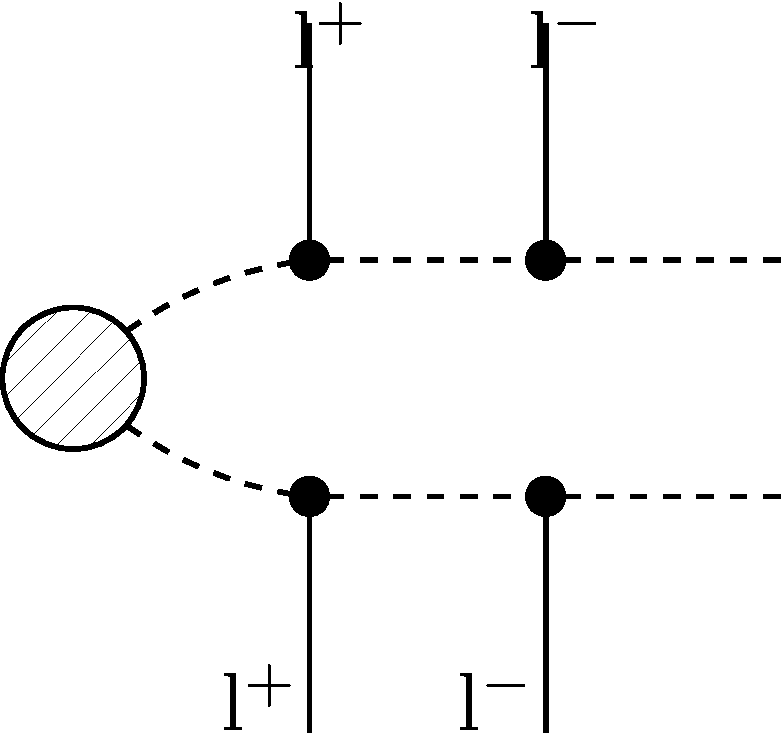
\includegraphics[width=0.15\linewidth]{figures/ATLAS_CONF_2013_036:TChiChiSlepSlep_TChiChiSlepSlep_1_.pdf}\spacer+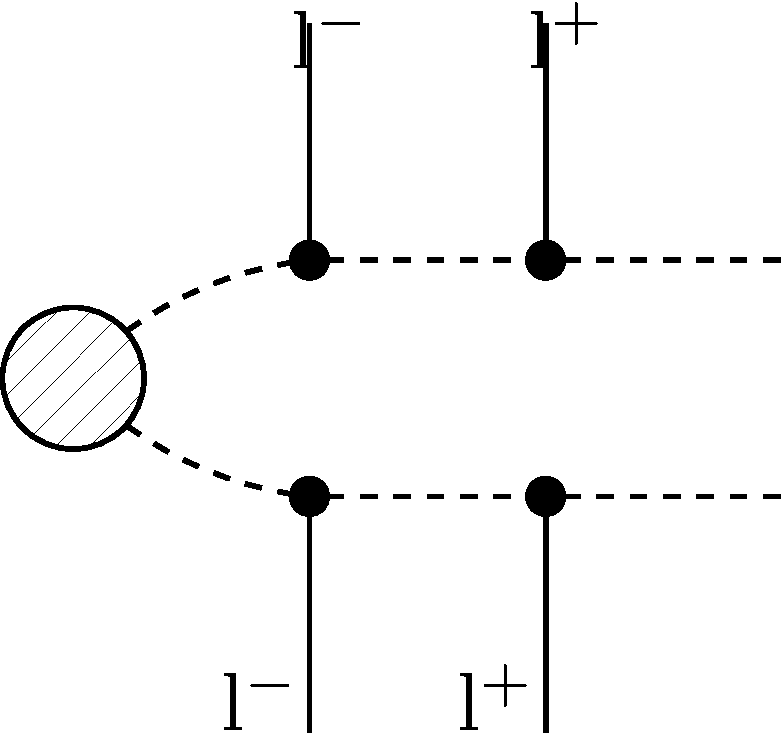
\includegraphics[width=0.15\linewidth]{figures/ATLAS_CONF_2013_036:TChiChiSlepSlep_TChiChiSlepSlep_2_.pdf}\spacer+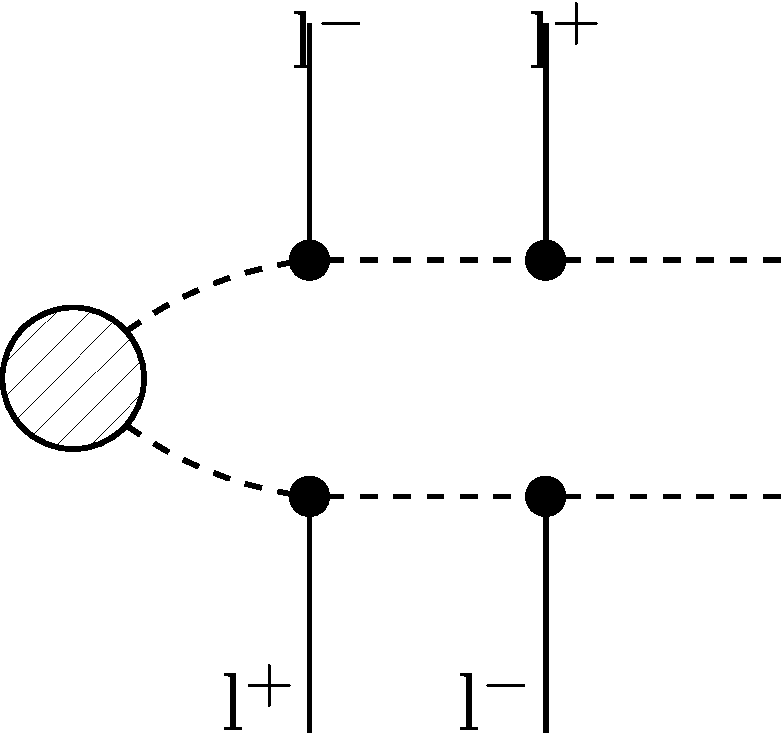
\includegraphics[width=0.15\linewidth]{figures/ATLAS_CONF_2013_036:TChiChiSlepSlep_TChiChiSlepSlep_3_.pdf}\spacer \\  \hline 
\multirow{2}{*}{ATLAS-CONF-2013-037 } &  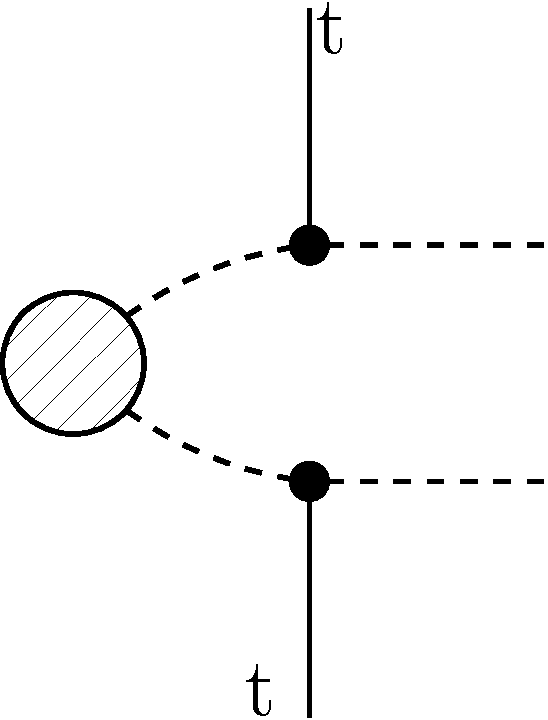
\includegraphics[width=0.15\linewidth]{figures/ATLAS_CONF_2013_037:T2tt_T2tt_1_.pdf}\spacer \\ 
 &  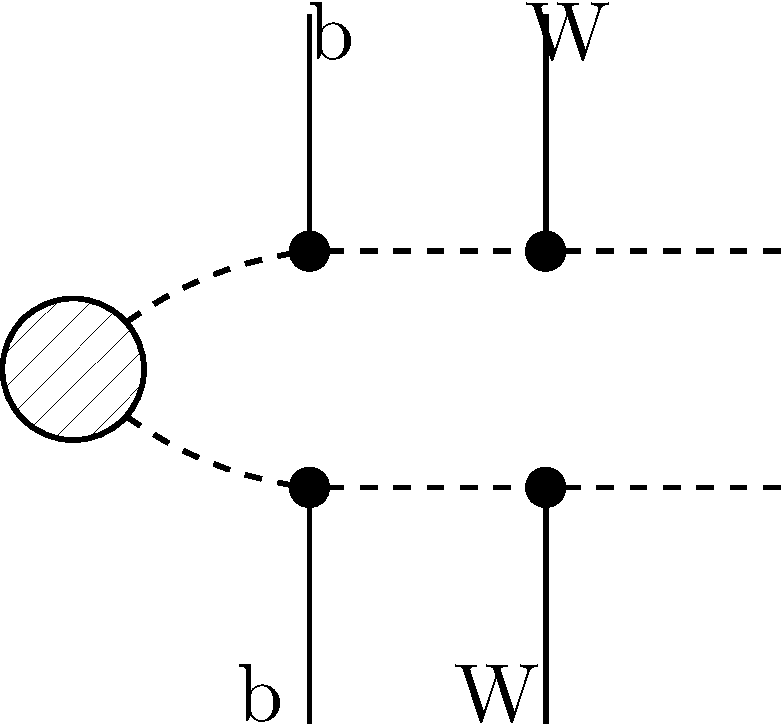
\includegraphics[width=0.15\linewidth]{figures/ATLAS_CONF_2013_037:T6bbWW_T6bbWW_1_.pdf}\spacer \\  \hline 
\multirow{1}{*}{ATLAS-CONF-2013-024 } &  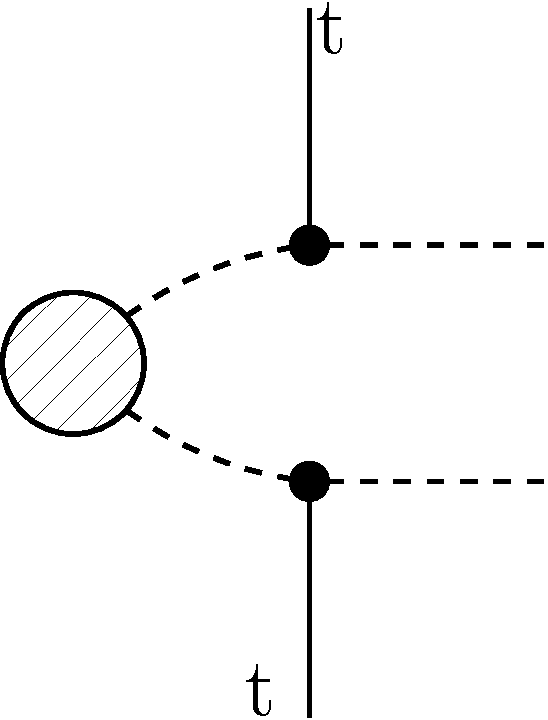
\includegraphics[width=0.15\linewidth]{figures/ATLAS_CONF_2013_024:T2tt_T2tt_1_.pdf}\spacer \\  \hline 
\multirow{1}{*}{MultiLepton8TeV } &  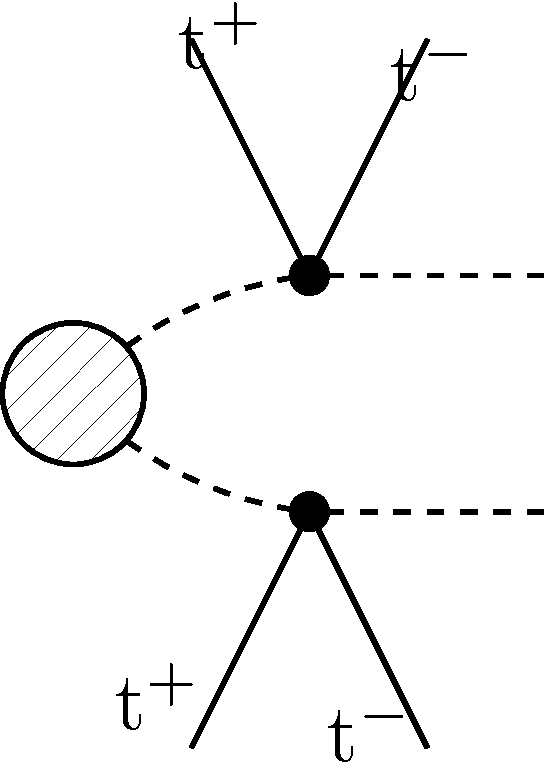
\includegraphics[width=0.15\linewidth]{figures/MultiLepton8TeV:T1tttt_T1tttt_1_.pdf}\spacer \\  \hline 
\multirow{2}{*}{LeptonicStop8TeV } &  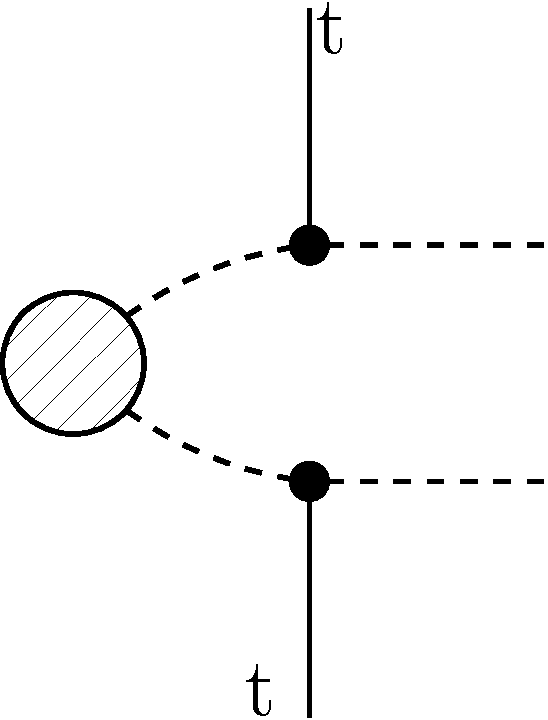
\includegraphics[width=0.15\linewidth]{figures/LeptonicStop8TeV:T2tt_T2tt_1_.pdf}\spacer \\ 
 &  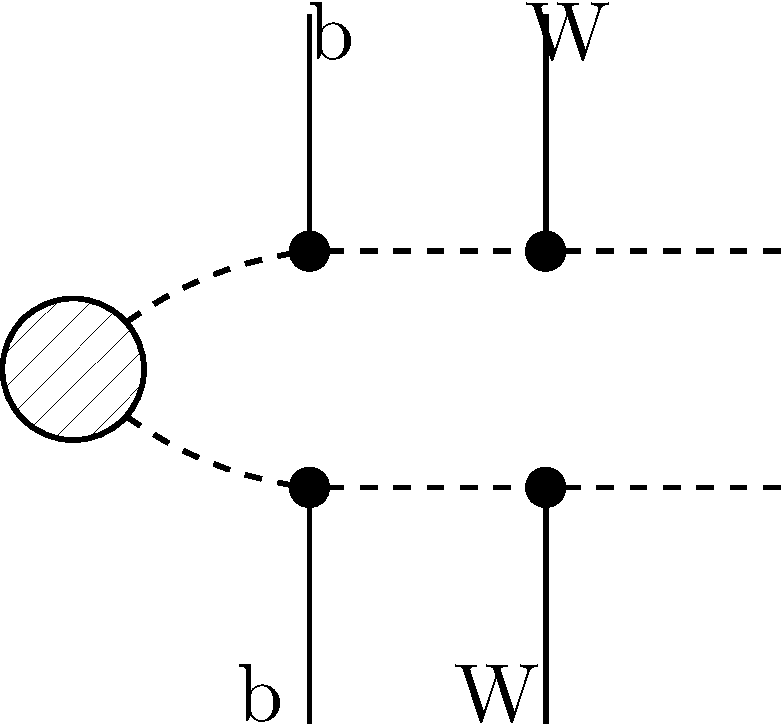
\includegraphics[width=0.15\linewidth]{figures/LeptonicStop8TeV:T6bbWW_T6bbWW_1_.pdf}\spacer \\  \hline 
\multirow{1}{*}{RA4LS8TeV } &  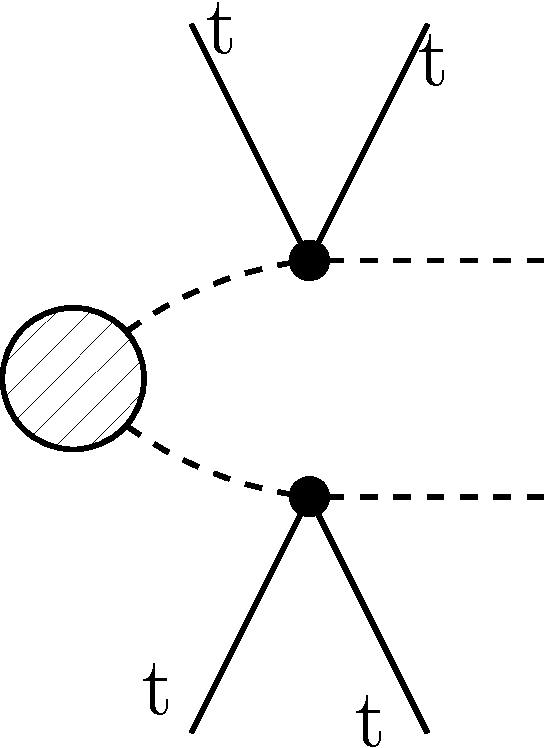
\includegraphics[width=0.15\linewidth]{figures/RA4LS8TeV:T1tttt_T1tttt_1_.pdf}\spacer \\  \hline 
\multirow{2}{*}{ATLAS-CONF-2013-035 } &  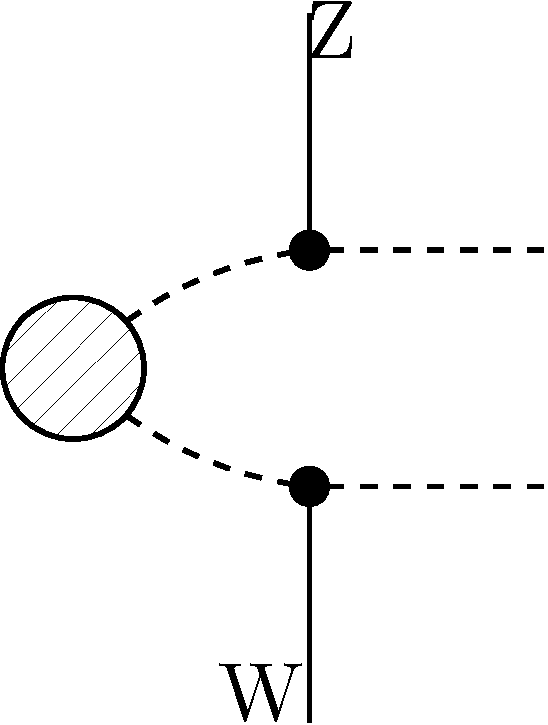
\includegraphics[width=0.15\linewidth]{figures/ATLAS_CONF_2013_035:TChiWZ_TChiWZ_1_.pdf}\spacer \\ 
 &  2.*(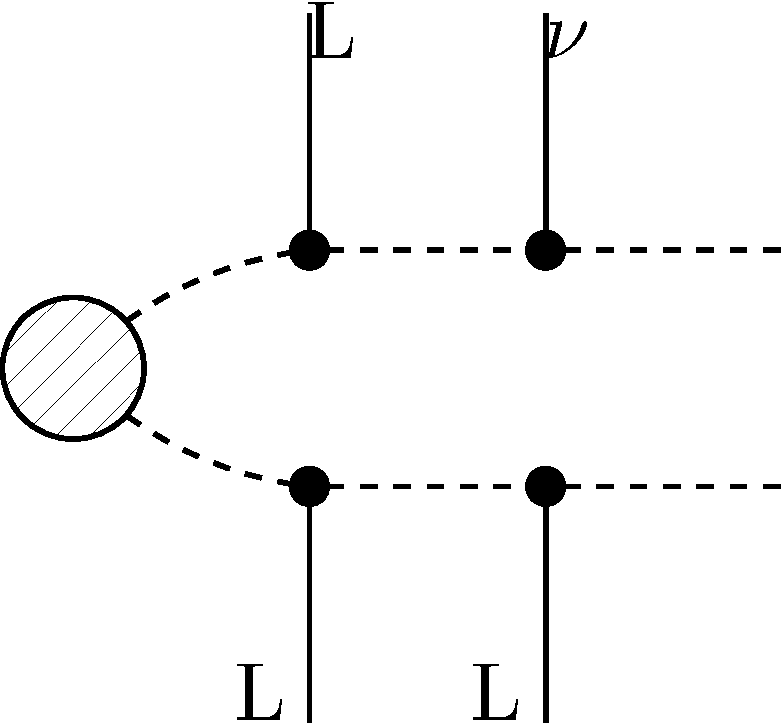
\includegraphics[width=0.15\linewidth]{figures/ATLAS_CONF_2013_035:TChiChipmSlepL_TChiChipmSlepL_1_.pdf}\spacer+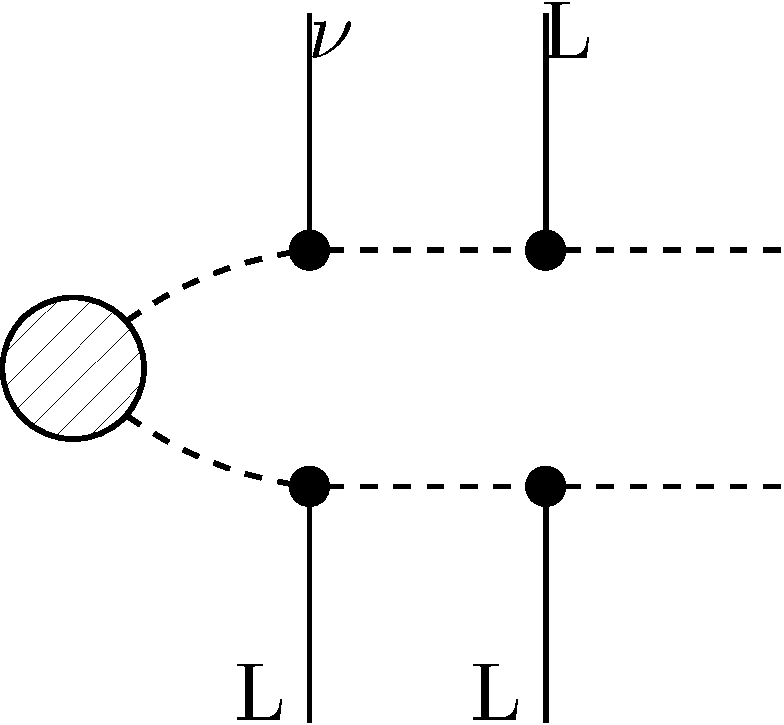
\includegraphics[width=0.15\linewidth]{figures/ATLAS_CONF_2013_035:TChiChipmSlepL_TChiChipmSlepL_2_.pdf}\spacer) \\  \hline 
\multirow{2}{*}{ATLAS-CONF-2012-166 } &  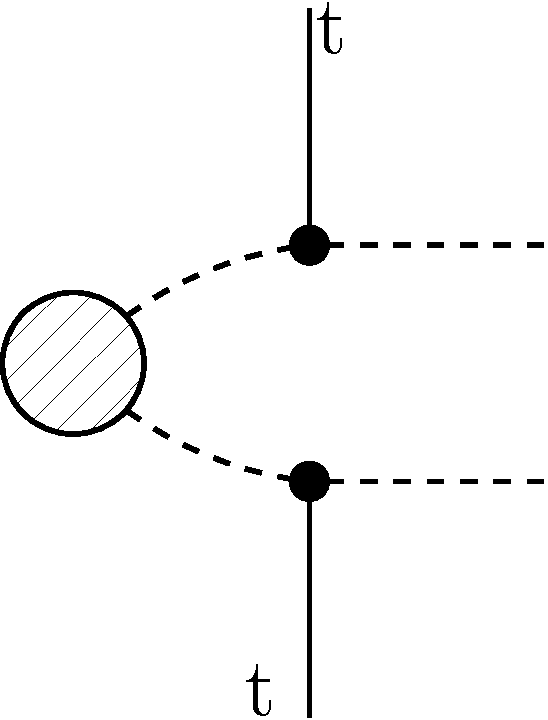
\includegraphics[width=0.15\linewidth]{figures/ATLAS_CONF_2012_166:T2tt_T2tt_1_.pdf}\spacer \\ 
 &  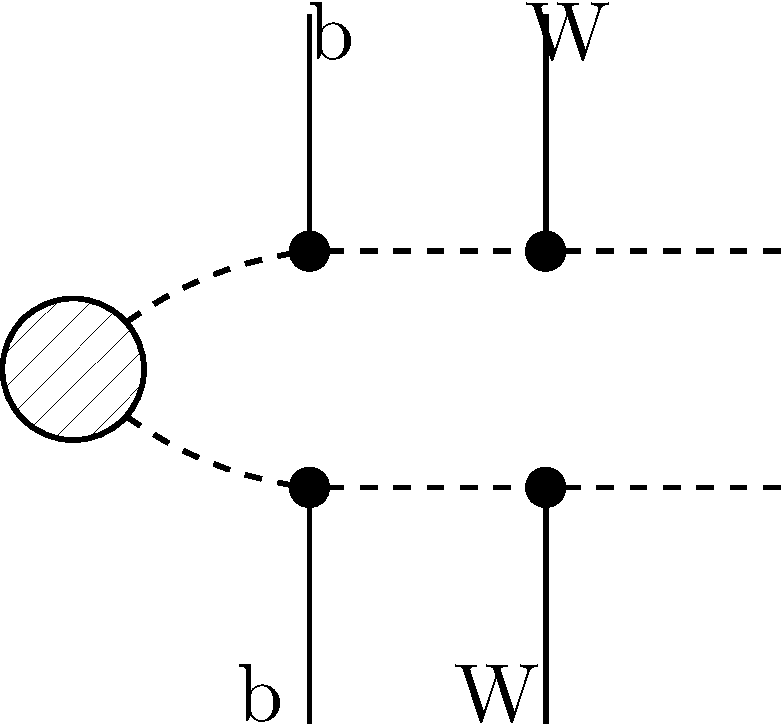
\includegraphics[width=0.15\linewidth]{figures/ATLAS_CONF_2012_166:T6bbWW_T6bbWW_1_.pdf}\spacer \\  \hline 
\multirow{1}{*}{ATLAS-CONF-2013-025 } &  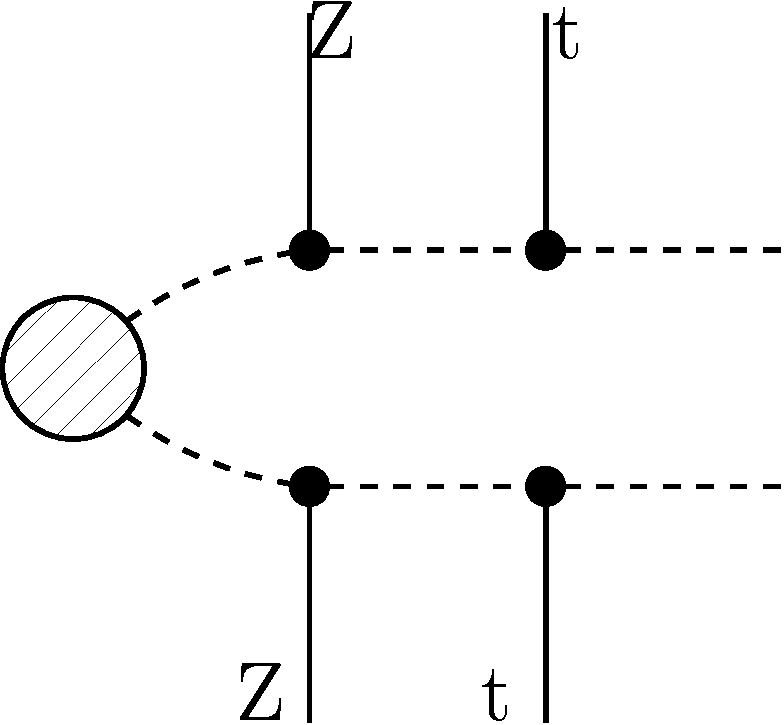
\includegraphics[width=0.15\linewidth]{figures/ATLAS_CONF_2013_025:T6ttZZ_T6ttZZ_1_.pdf}\spacer \\  \hline 
\multirow{6}{*}{alphaT } &  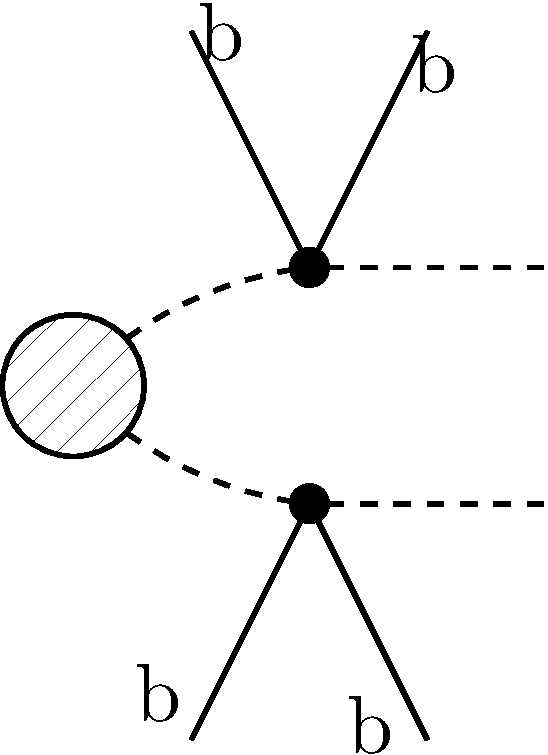
\includegraphics[width=0.15\linewidth]{figures/alphaT:T1bbbb_T1bbbb_1_.pdf}\spacer \\ 
 &  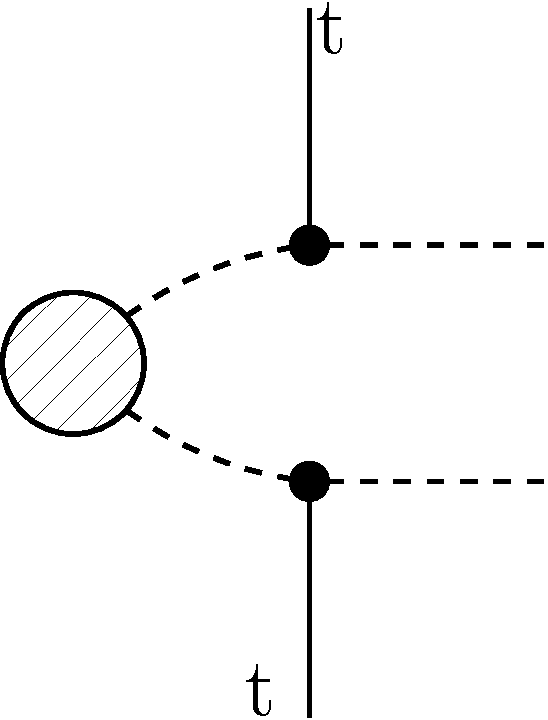
\includegraphics[width=0.15\linewidth]{figures/alphaT:T2tt_T2tt_1_.pdf}\spacer \\ 
 &  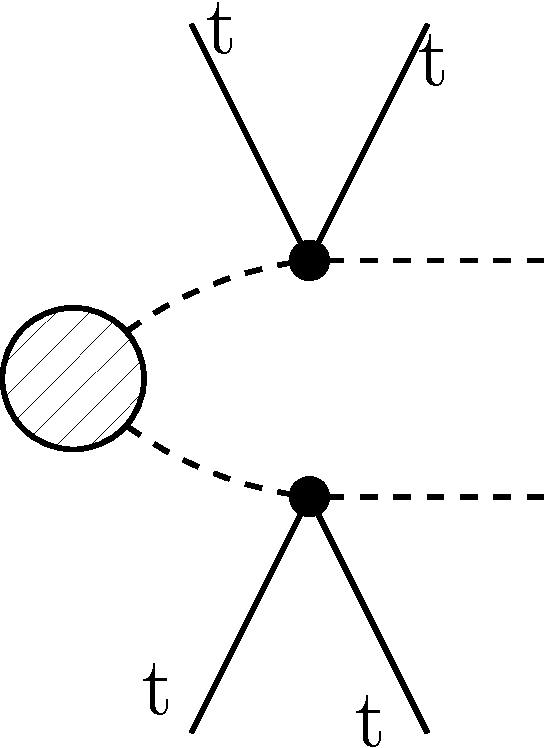
\includegraphics[width=0.15\linewidth]{figures/alphaT:T1tttt_T1tttt_1_.pdf}\spacer \\ 
 &  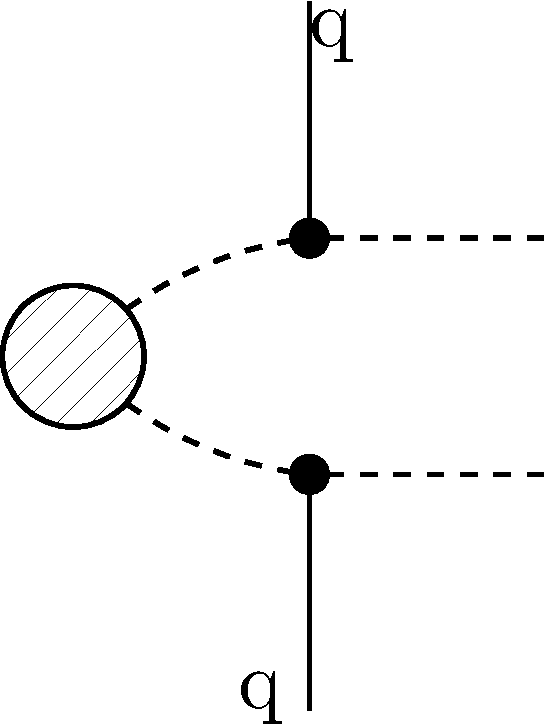
\includegraphics[width=0.15\linewidth]{figures/alphaT:T2_T2_1_.pdf}\spacer \\ 
 &  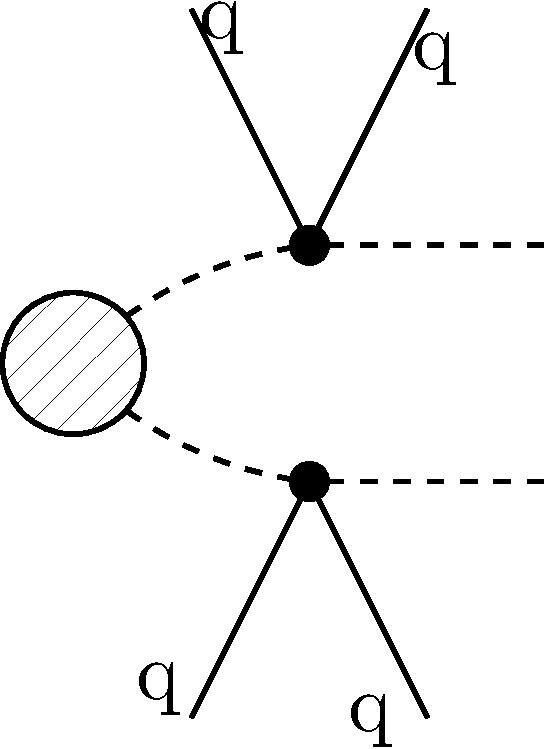
\includegraphics[width=0.15\linewidth]{figures/alphaT:T1_T1_1_.pdf}\spacer \\ 
 &  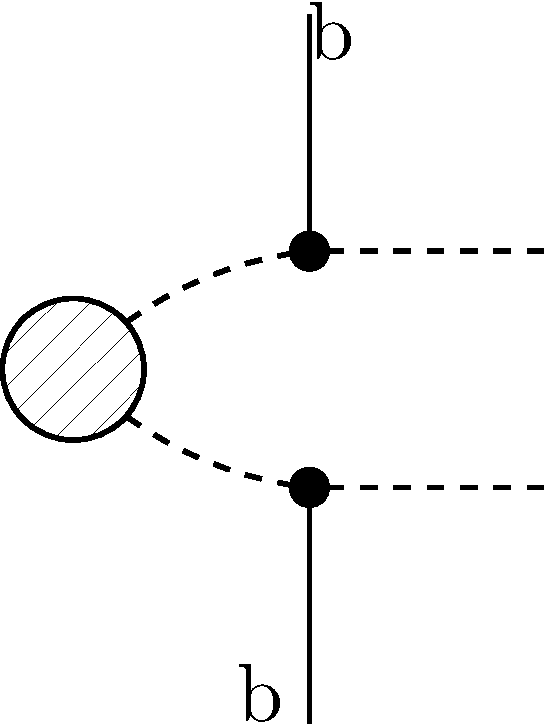
\includegraphics[width=0.15\linewidth]{figures/alphaT:T2bb_T2bb_1_.pdf}\spacer \\  \hline 
\multirow{1}{*}{ATLAS-CONF-2013-001 } &  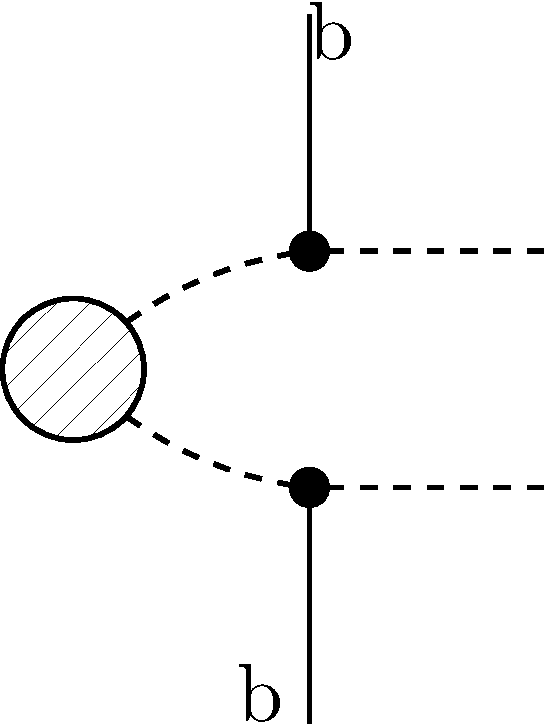
\includegraphics[width=0.15\linewidth]{figures/ATLAS_CONF_2013_001:T2bb_T2bb_1_.pdf}\spacer \\  \hline 
\multirow{5}{*}{ATLAS-CONF-2013-007 } &  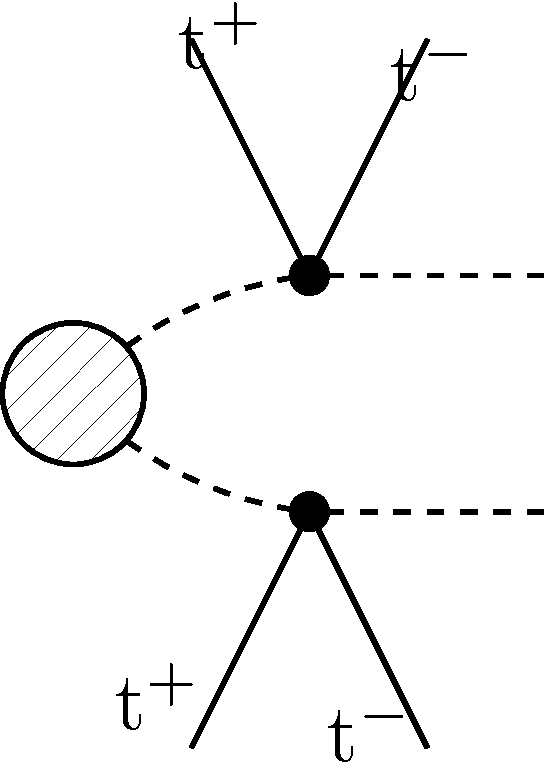
\includegraphics[width=0.15\linewidth]{figures/ATLAS_CONF_2013_007:T1tttt_T1tttt_1_.pdf}\spacer \\ 
 &  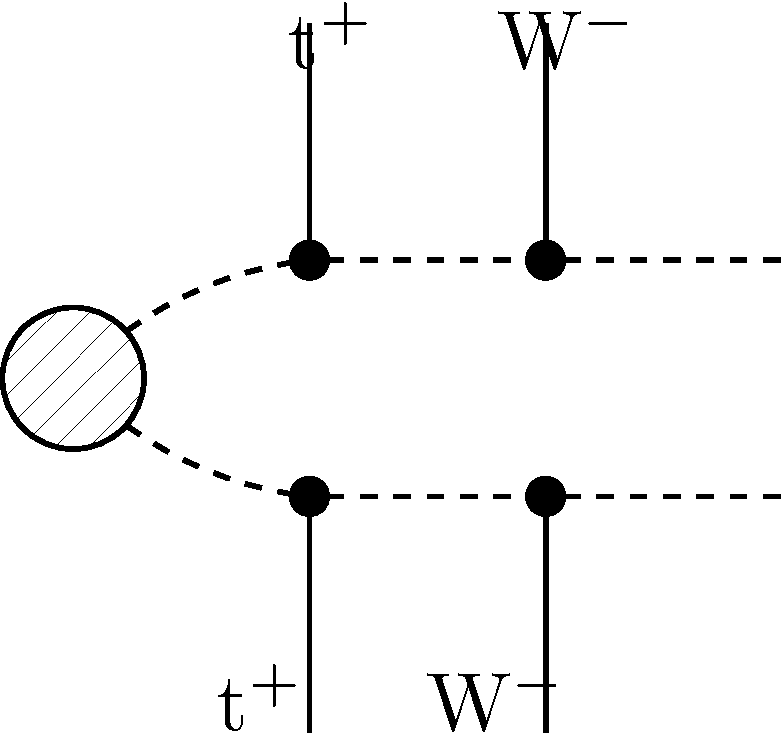
\includegraphics[width=0.15\linewidth]{figures/ATLAS_CONF_2013_007:T6ttWW_T6ttWW_1_.pdf}\spacer+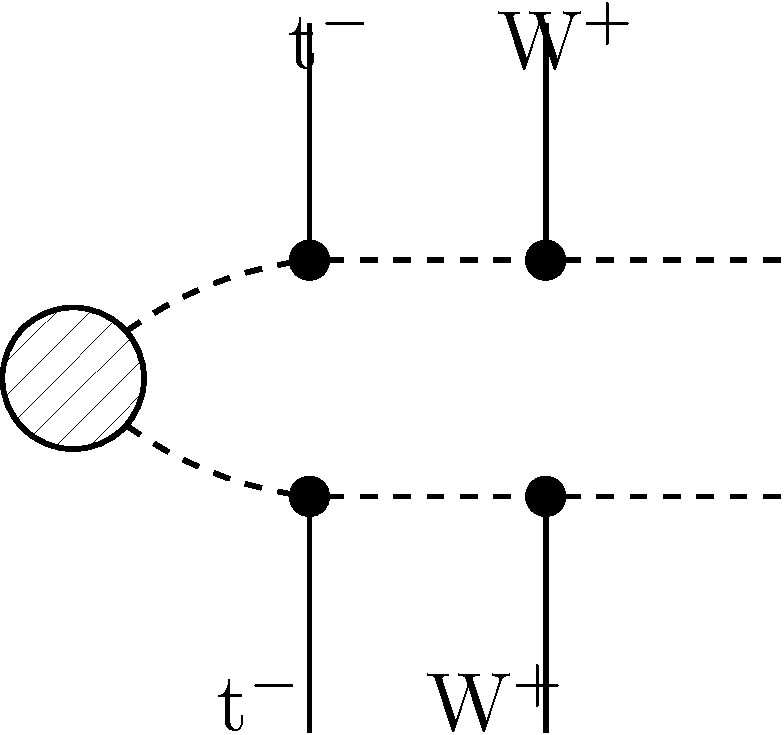
\includegraphics[width=0.15\linewidth]{figures/ATLAS_CONF_2013_007:T6ttWW_T6ttWW_2_.pdf}\spacer+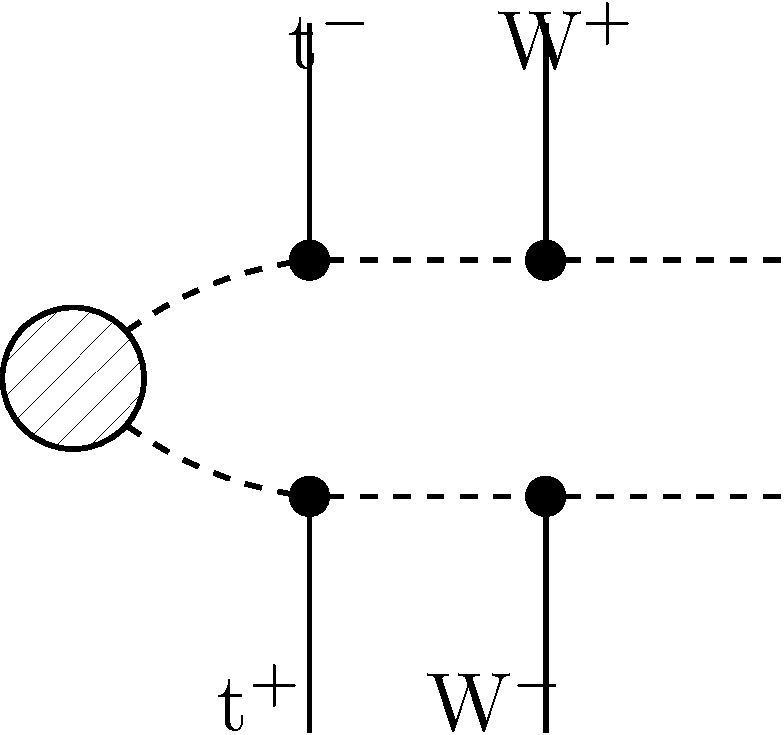
\includegraphics[width=0.15\linewidth]{figures/ATLAS_CONF_2013_007:T6ttWW_T6ttWW_3_.pdf}\spacer \\ 
 &  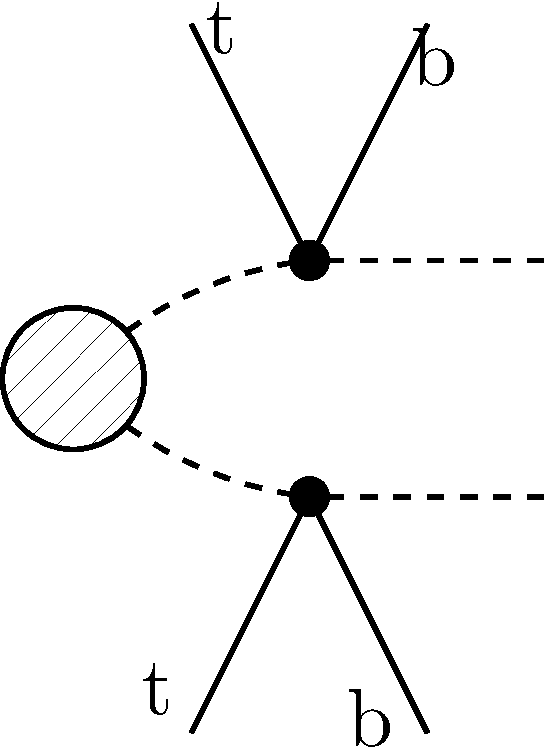
\includegraphics[width=0.15\linewidth]{figures/ATLAS_CONF_2013_007:T1tbtb_T1tbtb_1_.pdf}\spacer \\ 
 &  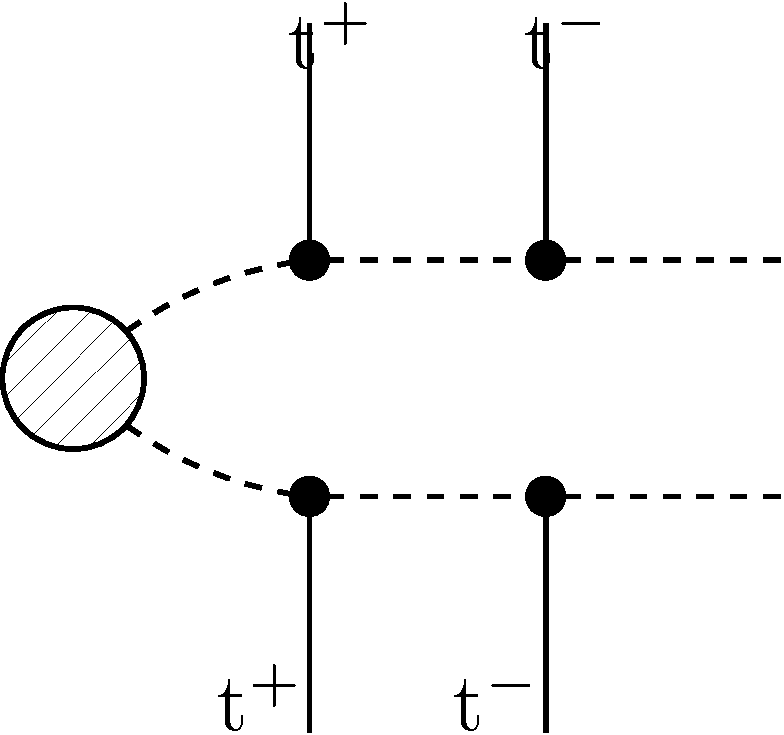
\includegraphics[width=0.15\linewidth]{figures/ATLAS_CONF_2013_007:T5tttt_T5tttt_1_.pdf}\spacer+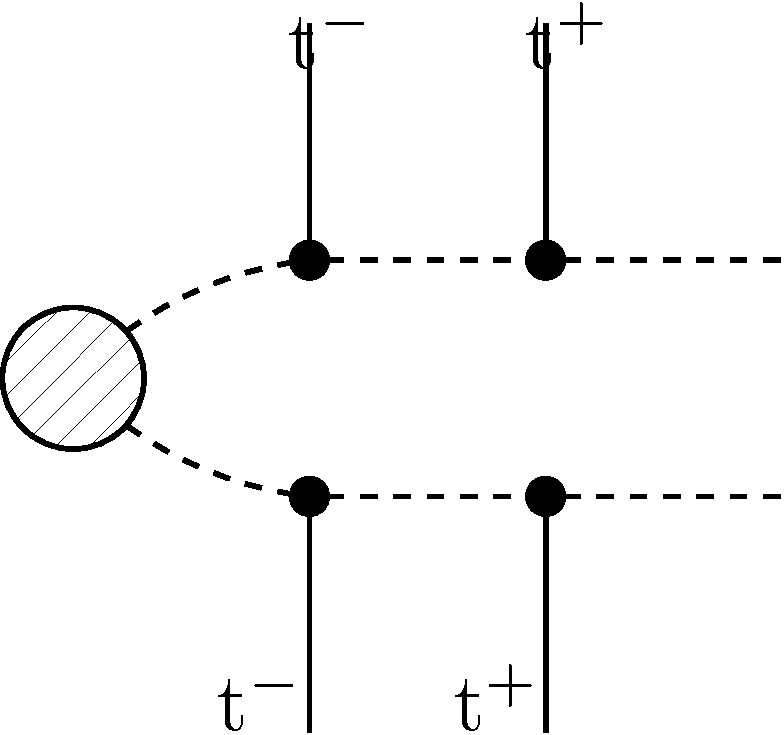
\includegraphics[width=0.15\linewidth]{figures/ATLAS_CONF_2013_007:T5tttt_T5tttt_2_.pdf}\spacer+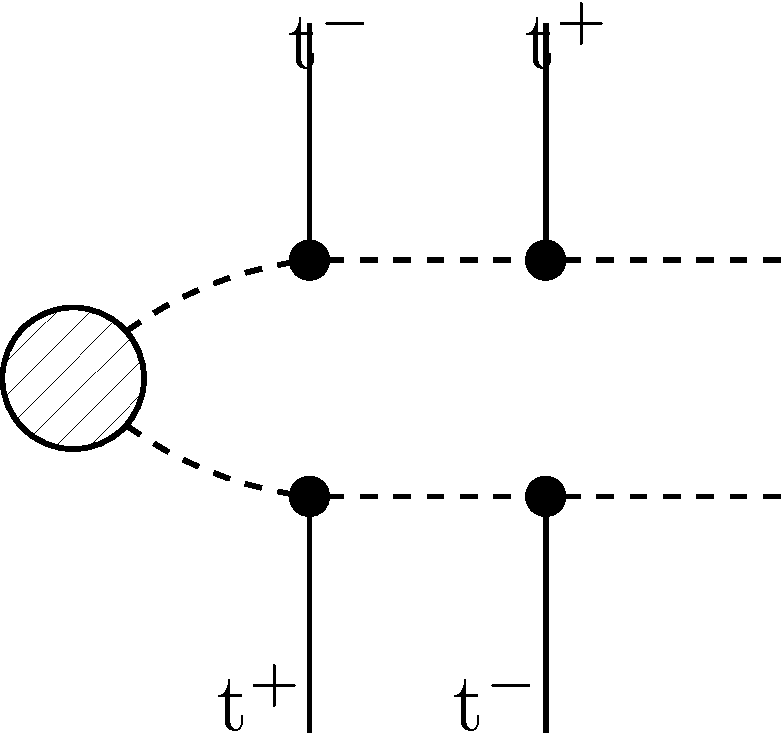
\includegraphics[width=0.15\linewidth]{figures/ATLAS_CONF_2013_007:T5tttt_T5tttt_3_.pdf}\spacer \\ 
 &  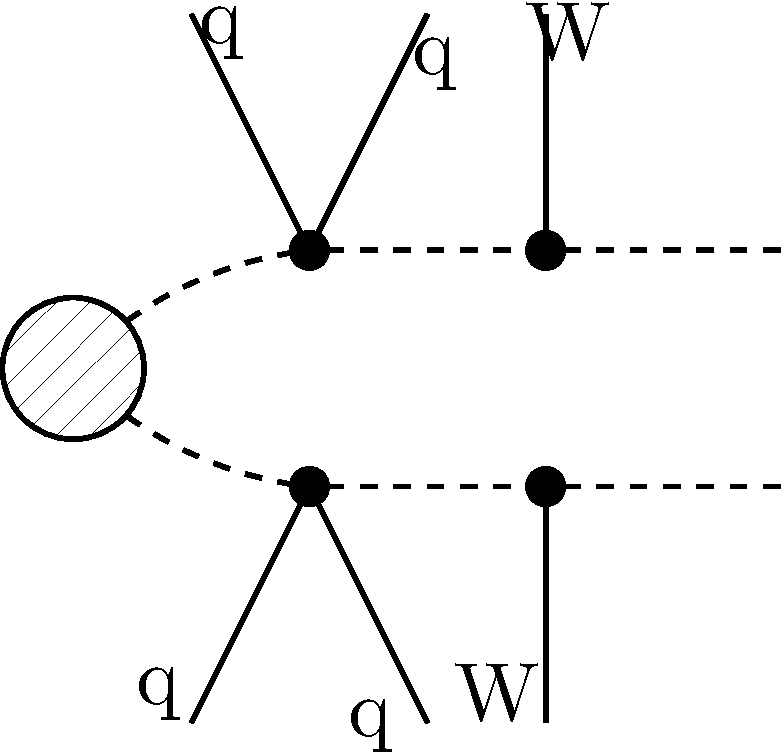
\includegraphics[width=0.15\linewidth]{figures/ATLAS_CONF_2013_007:T5WW_T5WW_1_.pdf}\spacer \\  \hline 
\multirow{2}{*}{ATLAS-CONF-2013-028 } &  2.*(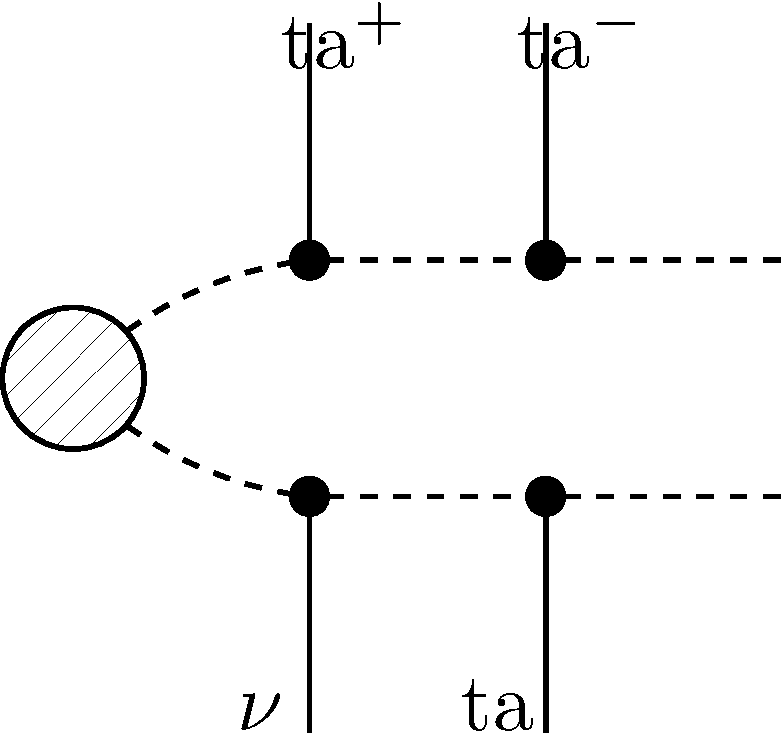
\includegraphics[width=0.15\linewidth]{figures/ATLAS_CONF_2013_028:TChiChipmStauL_TChiChipmStauL_1_.pdf}\spacer+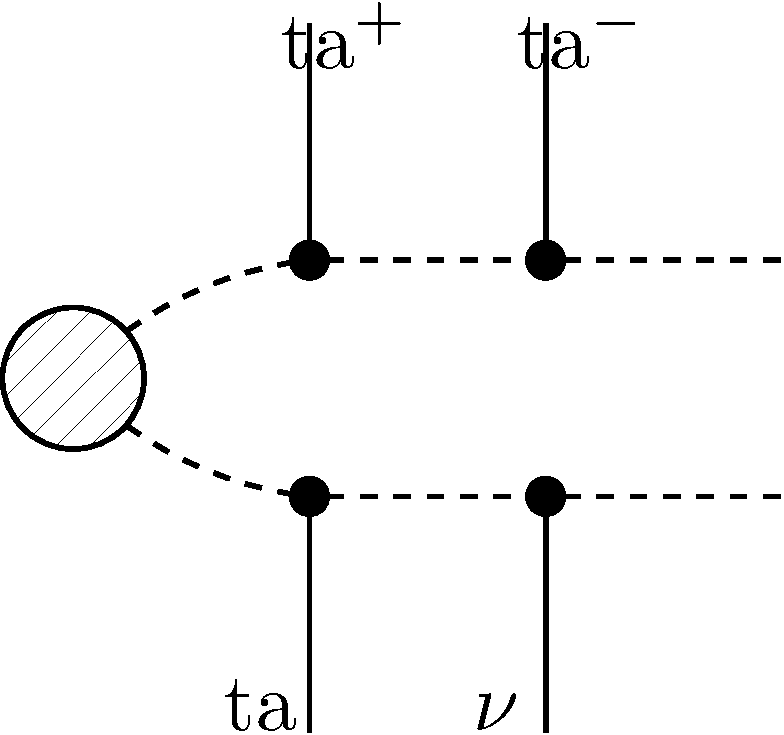
\includegraphics[width=0.15\linewidth]{figures/ATLAS_CONF_2013_028:TChiChipmStauL_TChiChipmStauL_2_.pdf}\spacer+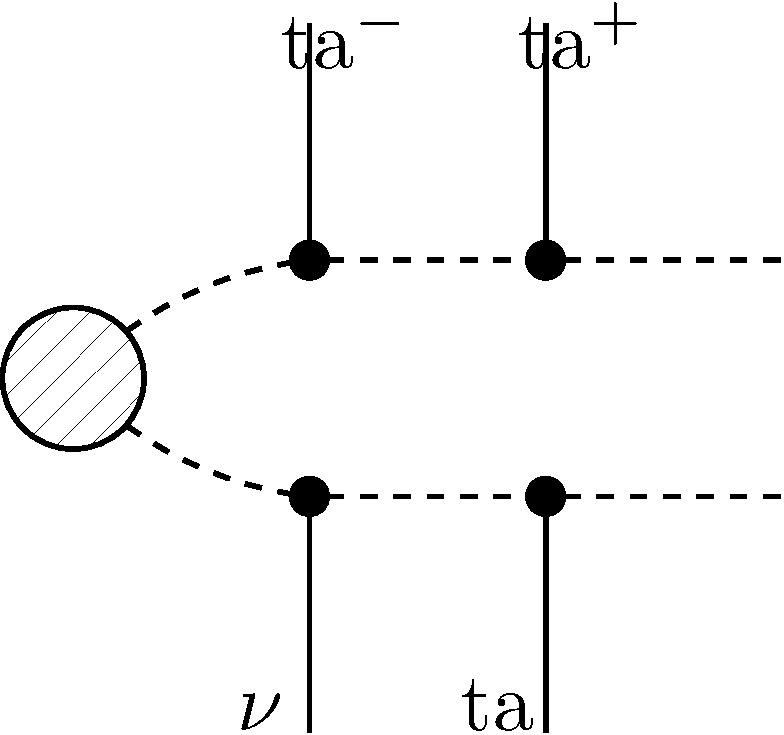
\includegraphics[width=0.15\linewidth]{figures/ATLAS_CONF_2013_028:TChiChipmStauL_TChiChipmStauL_3_.pdf}\spacer+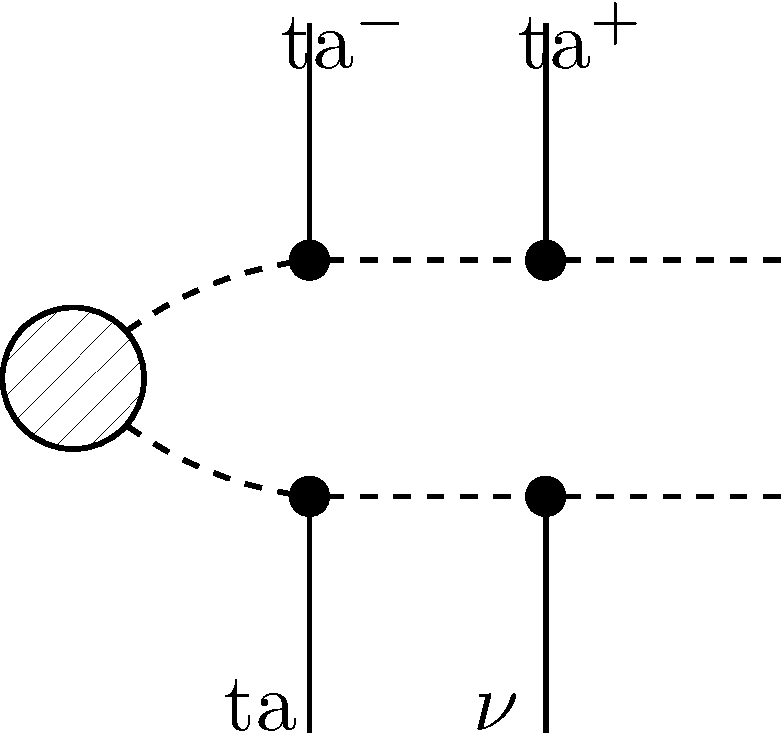
\includegraphics[width=0.15\linewidth]{figures/ATLAS_CONF_2013_028:TChiChipmStauL_TChiChipmStauL_4_.pdf}\spacer) \\ 
 &  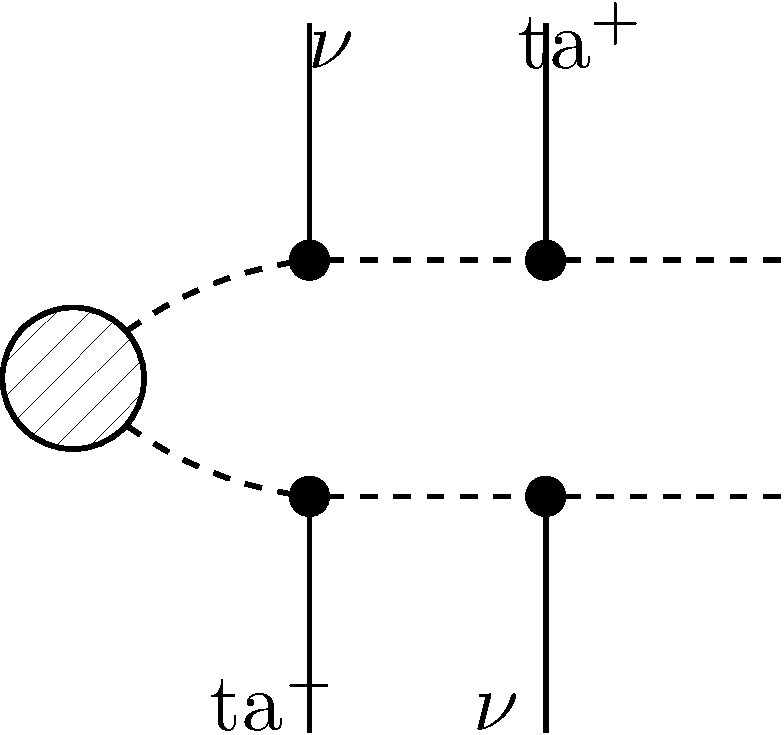
\includegraphics[width=0.15\linewidth]{figures/ATLAS_CONF_2013_028:TChipChimStauSnu_TChipChimStauSnu_1_.pdf}\spacer+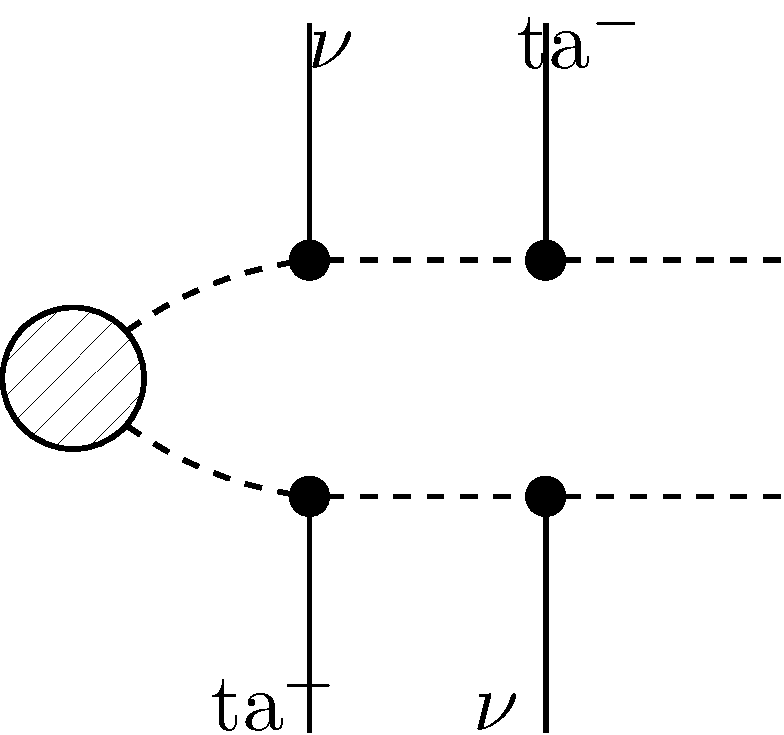
\includegraphics[width=0.15\linewidth]{figures/ATLAS_CONF_2013_028:TChipChimStauSnu_TChipChimStauSnu_2_.pdf}\spacer+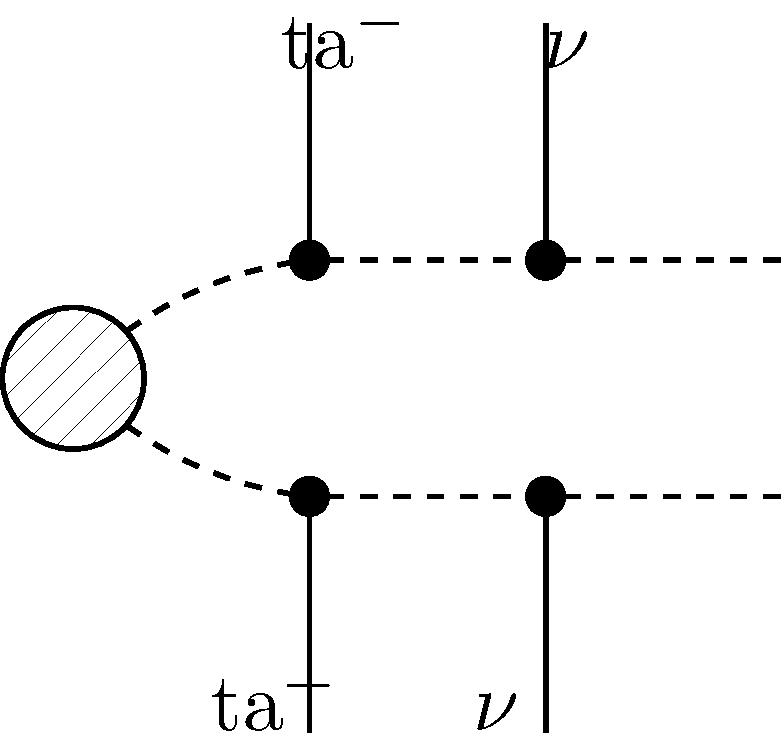
\includegraphics[width=0.15\linewidth]{figures/ATLAS_CONF_2013_028:TChipChimStauSnu_TChipChimStauSnu_3_.pdf}\spacer+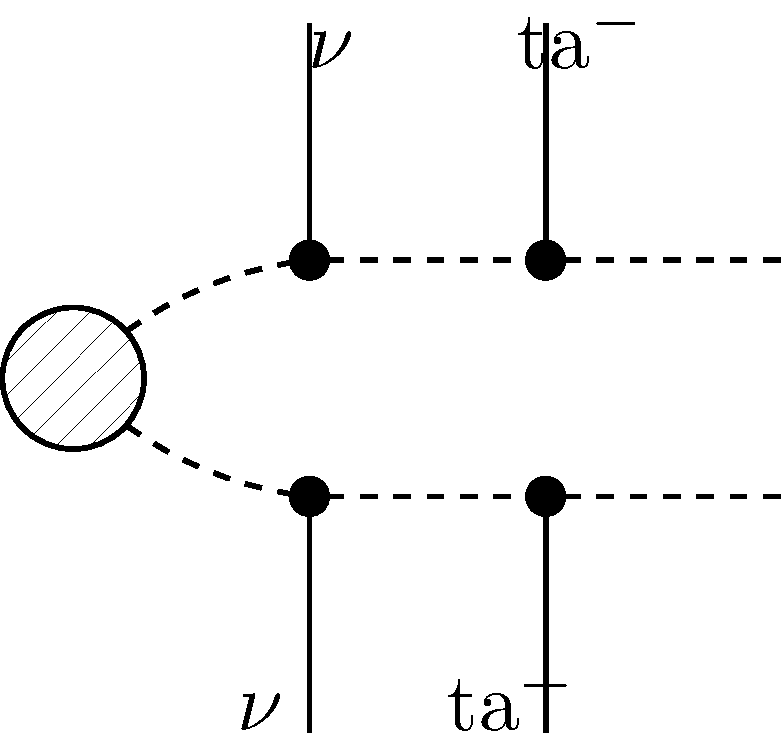
\includegraphics[width=0.15\linewidth]{figures/ATLAS_CONF_2013_028:TChipChimStauSnu_TChipChimStauSnu_4_.pdf}\spacer \\  \hline 
\multirow{6}{*}{Weakinos8TeV } &  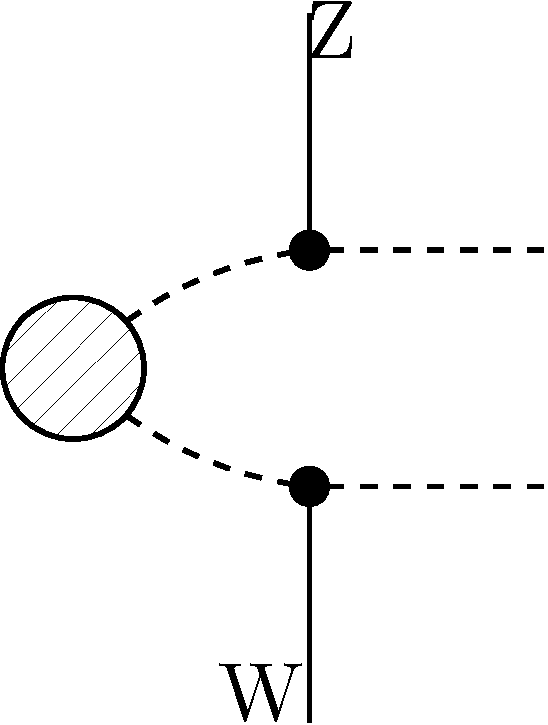
\includegraphics[width=0.15\linewidth]{figures/Weakinos8TeV:TChiWZ_TChiWZ_1_.pdf}\spacer \\ 
 &  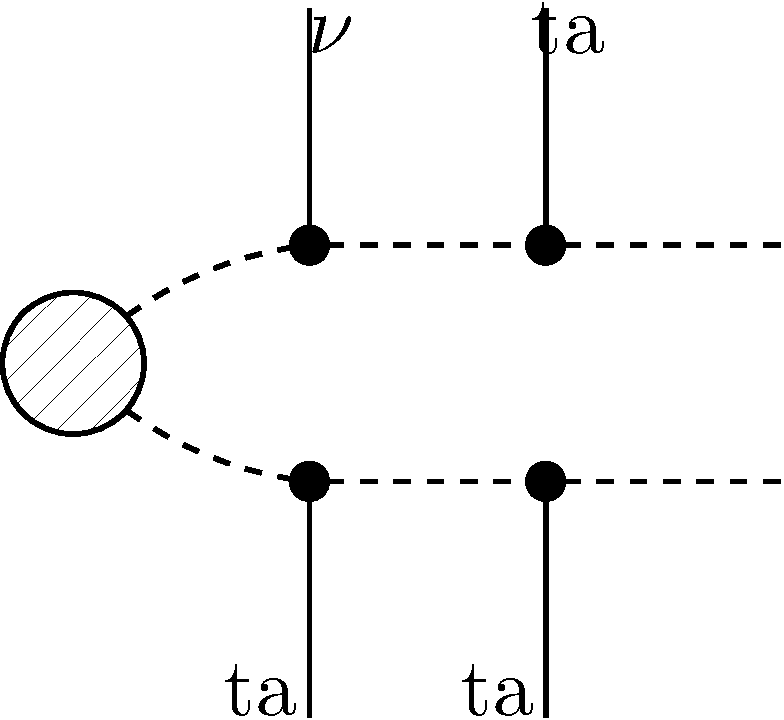
\includegraphics[width=0.15\linewidth]{figures/Weakinos8TeV:TChiChipmStauStau_TChiChipmStauStau_1_.pdf}\spacer \\ 
 &  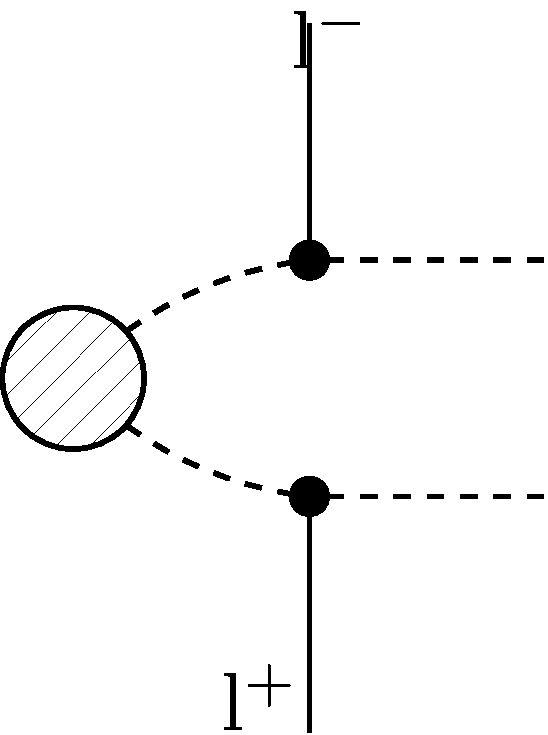
\includegraphics[width=0.15\linewidth]{figures/Weakinos8TeV:TSlepSlep_TSlepSlep_1_.pdf}\spacer \\ 
 &  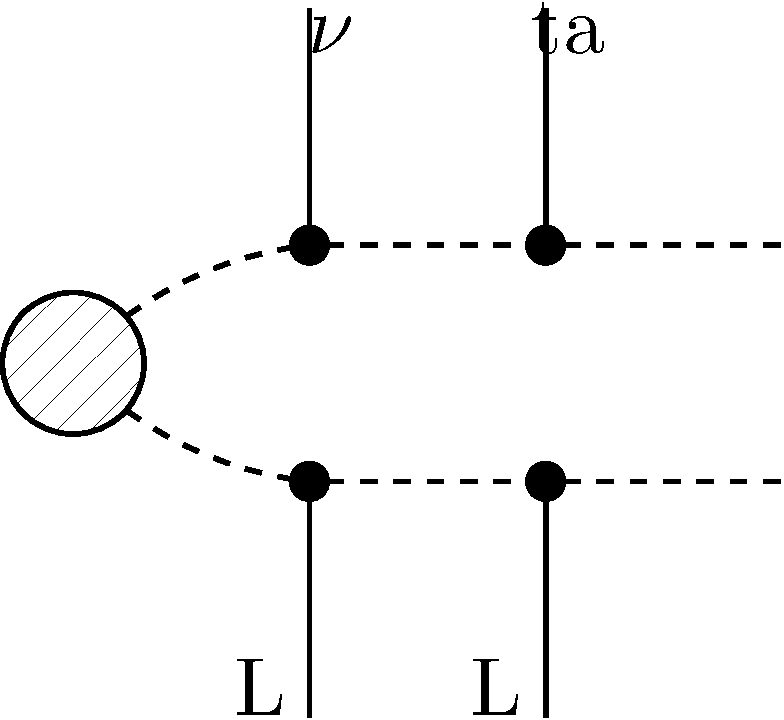
\includegraphics[width=0.15\linewidth]{figures/Weakinos8TeV:TChiChipmSlepStau_TChiChipmSlepStau_1_.pdf}\spacer \\ 
 &  2.*(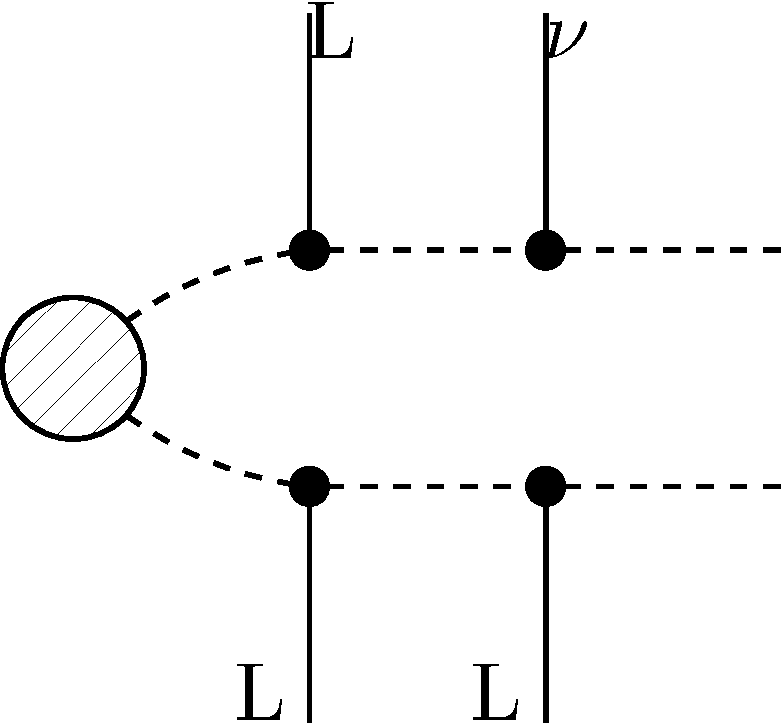
\includegraphics[width=0.15\linewidth]{figures/Weakinos8TeV:TChiChipmSlepL_TChiChipmSlepL_1_.pdf}\spacer+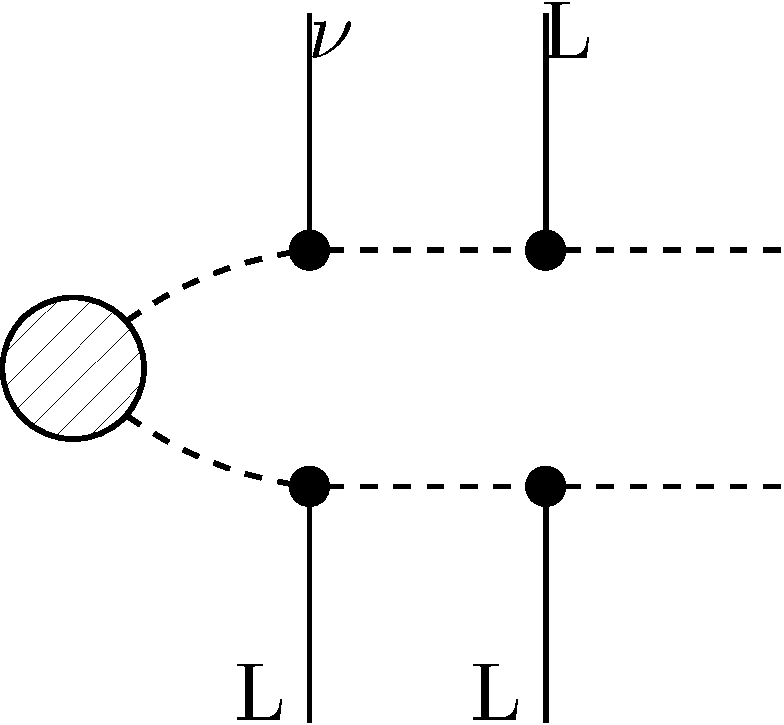
\includegraphics[width=0.15\linewidth]{figures/Weakinos8TeV:TChiChipmSlepL_TChiChipmSlepL_2_.pdf}\spacer) \\ 
 &  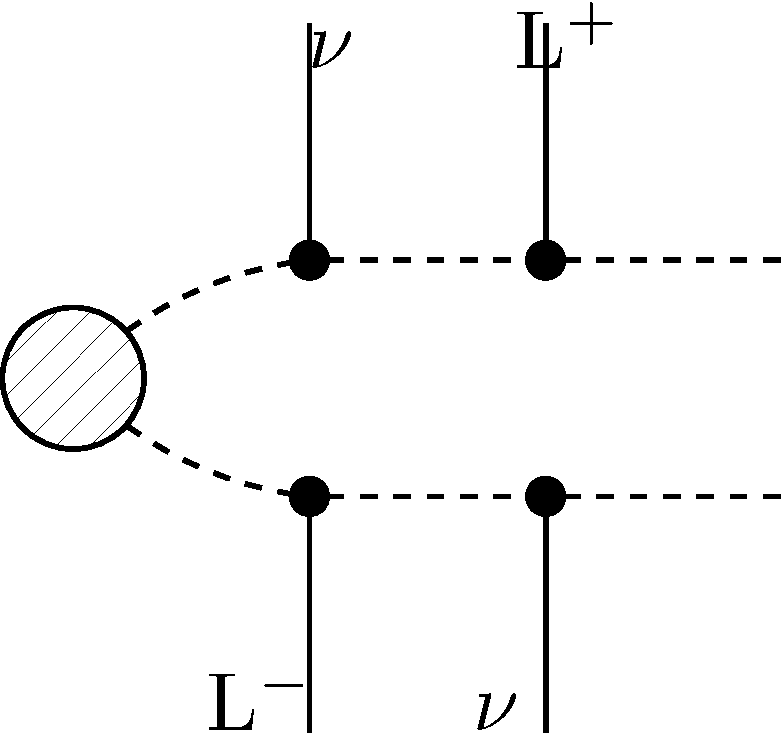
\includegraphics[width=0.15\linewidth]{figures/Weakinos8TeV:TChipChimSlepSnu_TChipChimSlepSnu_1_.pdf}\spacer+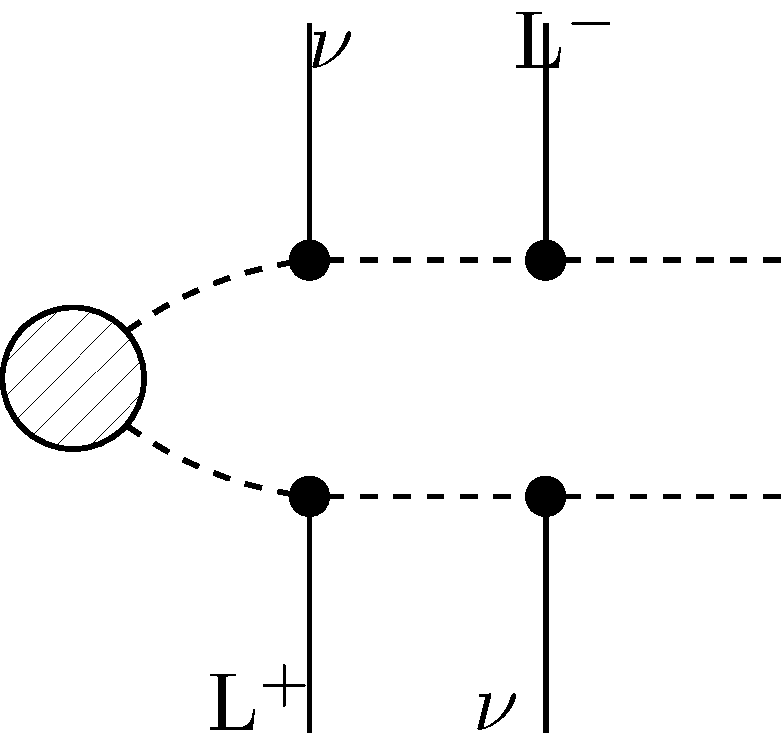
\includegraphics[width=0.15\linewidth]{figures/Weakinos8TeV:TChipChimSlepSnu_TChipChimSlepSnu_2_.pdf}\spacer+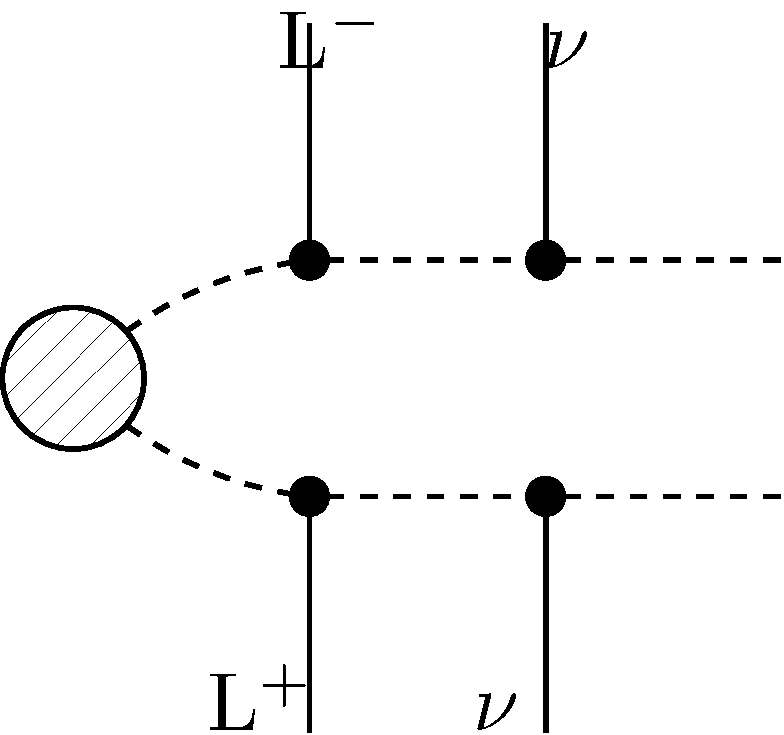
\includegraphics[width=0.15\linewidth]{figures/Weakinos8TeV:TChipChimSlepSnu_TChipChimSlepSnu_3_.pdf}\spacer+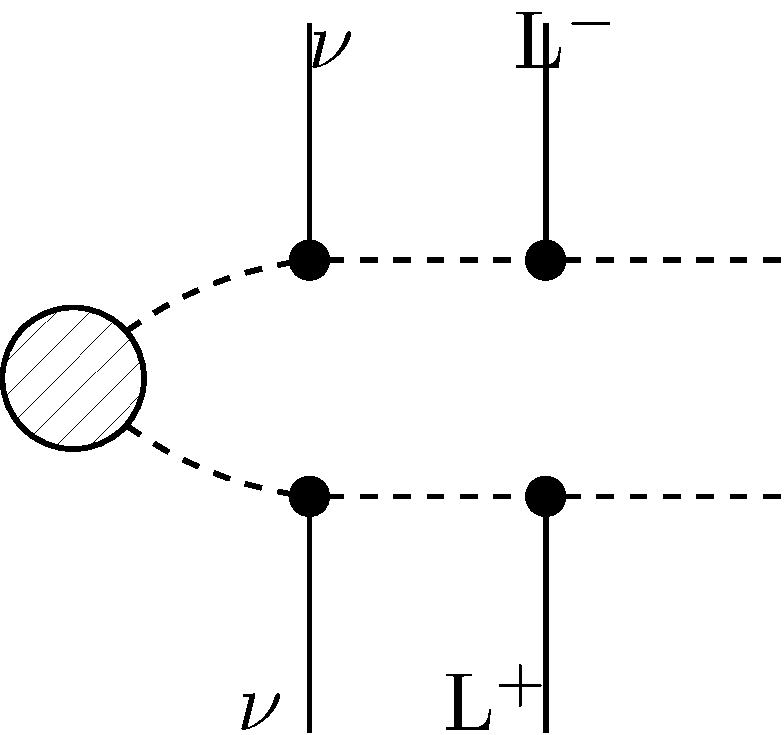
\includegraphics[width=0.15\linewidth]{figures/Weakinos8TeV:TChipChimSlepSnu_TChipChimSlepSnu_4_.pdf}\spacer \\  \hline 
\multirow{5}{*}{SUS13008 } &  \includegraphics[width=0.15\linewidth]{figures/SUS13008:T6ttWW_T6ttWW_1_.pdf}\spacer \\ 
 &  \includegraphics[width=0.15\linewidth]{figures/SUS13008:T1tttt_T1tttt_1_.pdf}\spacer \\ 
 &  \includegraphics[width=0.15\linewidth]{figures/SUS13008:T6bbZZ_T6bbZZ_1_.pdf}\spacer \\ 
 &  \includegraphics[width=0.15\linewidth]{figures/SUS13008:T7btbtWW_T7btbtWW_1_.pdf}\spacer \\ 
 &  \includegraphics[width=0.15\linewidth]{figures/SUS13008:T5tttt_T5tttt_1_.pdf}\spacer \\  \hline 
\multirow{2}{*}{RA2b8TeV } &  \includegraphics[width=0.15\linewidth]{figures/RA2b8TeV:T1bbbb_T1bbbb_1_.pdf}\spacer \\ 
 &  \includegraphics[width=0.15\linewidth]{figures/RA2b8TeV:T1tttt_T1tttt_1_.pdf}\spacer \\  \hline 
\multirow{6}{*}{alphaT8TeV } &  \includegraphics[width=0.15\linewidth]{figures/alphaT8TeV:T1bbbb_T1bbbb_1_.pdf}\spacer \\ 
 &  \includegraphics[width=0.15\linewidth]{figures/alphaT8TeV:T2tt_T2tt_1_.pdf}\spacer \\ 
 &  \includegraphics[width=0.15\linewidth]{figures/alphaT8TeV:T1tttt_T1tttt_1_.pdf}\spacer \\ 
 &  \includegraphics[width=0.15\linewidth]{figures/alphaT8TeV:T2_T2_1_.pdf}\spacer \\ 
 &  \includegraphics[width=0.15\linewidth]{figures/alphaT8TeV:T1_T1_1_.pdf}\spacer \\ 
 &  \includegraphics[width=0.15\linewidth]{figures/alphaT8TeV:T2bb_T2bb_1_.pdf}\spacer \\  \hline 
\multirow{1}{*}{ATLAS-CONF-2012-105 } &  \includegraphics[width=0.15\linewidth]{figures/ATLAS_CONF_2012_105:T1tttt_T1tttt_1_.pdf}\spacer \\  \hline 
\multirow{1}{*}{RA48TeV } &  \includegraphics[width=0.15\linewidth]{figures/RA48TeV:T1tttt_T1tttt_1_.pdf}\spacer \\  \hline 
\caption{LHC analyses included in our results. We also show the SMS topologies (or sums of topologies) constrained by each analysis\fixme{Just a rough idea.Definetely needs improvement}.} 
   \label{tab:LHCresults} 
   \end{longtable}

\FloatBarrier

